\section{Motivation}
\label{sec:classifiers-motivation}

We first describe how maximizing energy efficiency is distinct from maximizing performance or minimizing power consumption.
As such, finding the most energy-efficient system setting requires new techniques.
We then discuss the challenges of learning a model for mapping application/system behavior to energy-efficient system settings.


\subsection{Energy Efficiency is a Unique Challenge}

Energy efficiency is the ratio of work completed per unit of energy consumed.
For example, HPC clusters can formulate energy efficiency as the ratio of applications completed per Joule of energy used.
If an application execution represents some unit of scientific insight, then this metric expresses the cost of scientific insights in terms of operational costs (energy consumption).
Thus, maximizing energy efficiency directly reduces the cost of scientific insight by minimizing application energy consumption.

Some recent energy-aware approaches in HPC reduce energy consumption while maintaining application performance \cite{Jitter,Marathe2015,RountreeAdagio}.
As these approaches do not trade application speed, they reduce energy strictly by reducing power.
While it is tempting to use the same approaches to minimize energy by simply removing the constraint on application runtime, failing to account for the impact of lower-power resource settings on execution time can result in worse energy consumption.
Also, while raising processor clockspeed typically reduces application runtime, the requisite increase in power results in increased energy consumption (recall \eqnref{bg-power} in \secref{intro-description}).
In short, maximizing energy efficiency \emph{does not} mean using as little power as possible \emph{or} running as fast as possible---it requires finding the optimal tradeoff between execution time and power consumption.


Typical resource management approaches in HPC clusters primarily attempt to optimize application completion time, only worrying about power consumption to the extent that the total cluster power constraint is not violated, and ignoring energy consumption altogether.
Although there are various techniques for assigning jobs to nodes, minimizing their runtime is usually achieved by running the individual compute nodes as fast as possible, \ie the \emph{race-to-idle} heuristic.
Using \emph{race-to-idle} makes resource scheduling on a node easy, but it is never as energy-efficient as a more intelligent approach that understands how system settings affect performance and power tradeoffs on a per-application basis \cite{kim-cpsna2015}.
\emph{Racing} to finish a job as fast as possible minimizes execution time, but the increase in power dwarfs the time savings, resulting in high energy consumption.

In addition to reducing costs, maximizing energy efficiency will also improve overall system throughput in power-constrained environments.
In over-provisioned clusters, the hardware can draw more total power than the infrastructure can physically deliver to the system if nodes use \emph{race-to-idle} \cite{Sarood2013}.
Effectively, power is now the primary factor limiting cluster size and throughput, not available compute resources.
More aggressively trading performance and power means that optimizing energy efficiency increases total cluster throughput by: (1) allowing more applications to run in parallel due to lower per-application power consumption, while (2) still considering application runtime due to its impact on energy consumption.
Therefore, new resource management approaches are required that focus solely on minimizing energy to reduce the cost of science (in Joules), even if application runtime is increased.


\subsection{Learning Energy Efficiency}
\label{sec:challenges-learning}

Identifying energy-efficient combinations of resource settings is challenging as there is no universal best setting for a system---it depends on the application and its configuration, even varying for different inputs.
Even in a parallel system with homogeneous nodes and perfectly uniform application behavior, optimal settings can vary dramatically due to manufacturing variation \cite{Acun2016}.
Furthermore, many applications progress through different \emph{phases} during execution.
For example, an application may transition between compute and memory-intensive processing, causing the most energy-efficient setting to change during runtime.
It is therefore not optimal to choose a single setting statically when launching the application, necessitating a dynamic approach instead.

We explore learning approaches that adjust system settings to minimize energy.
Specifically, we tune socket allocation, the use of HyperThreads, and processor DVFS.
The learning component picks settings for the combination of these resources such that, at any point during the application execution, the system is operating in its most energy-efficient state.

Our goal is for the learner to find the most energy-efficient setting without requiring any application-level changes.
We therefore use existing hardware performance counters as \emph{features}.
The learner then determines a function that maps some subset of these features into the most energy-efficient system setting.
However, system settings in modern compute nodes have very complicated interactions, so it is essential to use learning mechanisms that can produce accurate mappings despite this complexity.

\begin{figure}[t]
% \vskip -1.0em
\centering
\subfloat[Training data only.]
{\centering 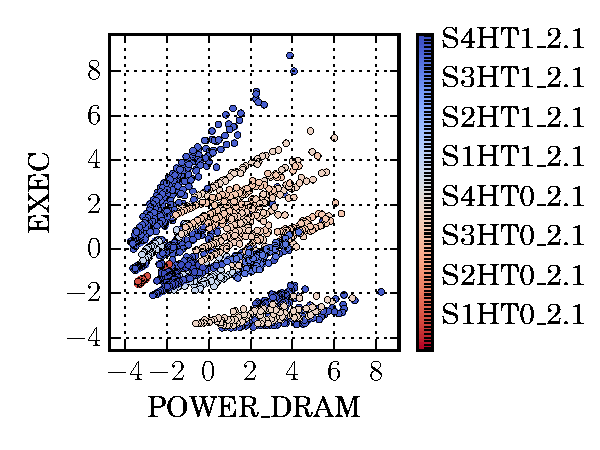
\includegraphics[width=0.3\columnwidth]{figs/classifiers/training_space_noclassifier.pdf}
\label{fig:feat-space-none}
% \vspace{ -1.5em }
}
\hspace*{0.1cm}
% \vskip -1.5em
\subfloat[SVM (Linear kernel), recall=0.456.]
{\centering 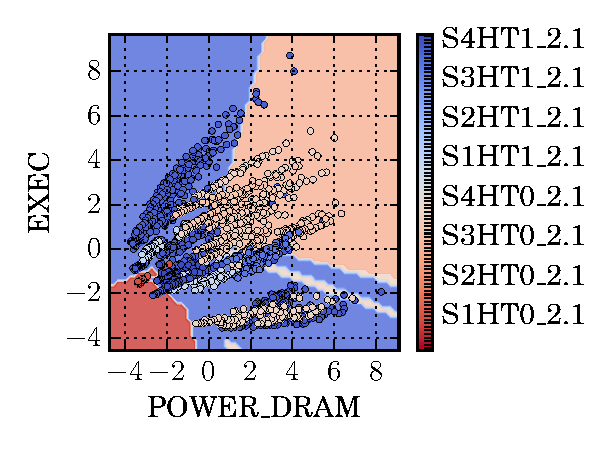
\includegraphics[width=0.3\columnwidth]{figs/classifiers/training_space_svm_kern_lin.pdf}
\label{fig:feat-space-svm-kern-lin}
% \vspace{ -1.5em }
}
\hspace*{0.1cm}
\subfloat[SVM (RBF kernel), recall=0.710.]
{\centering 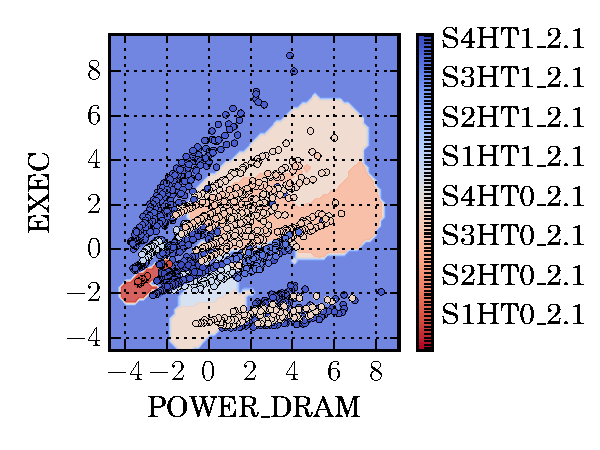
\includegraphics[width=0.3\columnwidth]{figs/classifiers/training_space_svm.pdf}
\label{fig:feat-space-svm}
% \vspace{ -1.5em }
}
\caption{Training data and learned decision boundaries for two SVM classifiers using two primary features.}
\label{fig:feat-space-intro}
% \vskip -1.0em
\end{figure}

We briefly illustrate this complexity using just two features---the performance counters \pc{POWER\_DRAM} (a measure of memory usage) and \pc{EXEC} (a measure of CPU usage).
\figref{feat-space-none} visualizes the behavior of our training data (21 common HPC benchmarks) with respect to normalized performance counter values.
Each data point is the average recorded \pc{POWER\_DRAM} and \pc{EXEC} behavior for a training application running in a single resource configuration on our evaluation system.
There are 88 unique resource configurations, or possible \emph{labels}, accounting for different combinations of the socket count \texttt{S}, whether HyperThreads \texttt{HT} are used, and the DVFS frequency (\eg 2.1\GHz).
% Thus, each application has 88 data points.
All 88 data points belonging to a particular application are assigned \emph{the same label}---the resource configuration with the best average energy efficiency for that application; \ie all 88 data points for an application have the same color.
With this labeling, a good learner will recognize suboptimal behavior and produce the most energy-efficient settings to use instead.
The problem is clearly complex---no intuitive pattern emerges that obviously maps CPU and memory usage into the most energy-efficient system settings.

To successfully map these features into accurate predictions, the learner must be able to handle this complexity, which not all learning mechanisms can.
Consider \figref{feat-space-svm-kern-lin}, which illustrates the accuracy of a Support Vector Machine (SVM) classifier using a linear kernel.
The shaded regions indicate the label (system settings) that the SVM classifier predicts for a range of feature values; the training data is overlaid for comparison.
This linear SVM's \emph{recall}---the fraction of system settings that are accurately predicted when simply replaying the training data---is only 45.6\%, a clear indication that this classifier is not effective.
In contrast, \figref{feat-space-svm} demonstrates a SVM with a radial basis function (RBF) kernel, which achieves 71.0\% recall---better, though perhaps still with room for further improvement.
Note that recall is simpler than cross-validation, since the classifier already saw the same input during supervised training.
If a classifier cannot perform accurate recall, it will likely perform even worse in deployment, when it is exposed to data it has not yet seen.
